\documentclass[
    iai, % Saisir le nom de l'institut rattaché
    eai, % Saisir le nom de l'orientation
    confidential, % Décommentez si le travail est confidentiel
]{heig-tb}

\usepackage[nooldvoltagedirection,european,americaninductors]{circuitikz}

\signature{mbernasconi.svg} % Remplacer par votre propre signature vectorielle.

\makenomenclature
\makenoidxglossaries
\makeindex

\addbibresource{bibliography.bib}



\nomenclature[A, 02]{\(c\)}{\href{https://physics.nist.gov/cgi-bin/cuu/Value?c}
  {Vitesse de la lumière dans le vide}
  \nomunit{\qty{299792458}{\meter\per\second}}}

\nomenclature[A, 03]{\(h\)}{\href{https://physics.nist.gov/cgi-bin/cuu/Value?h}
  {Constante de Planck}
  \nomunit{\qty[group-digits=none]{6.62607015e-34}{\joule\per\hertz}}}

\nomenclature[A, 01]{\(G\)}{\href{https://physics.nist.gov/cgi-bin/cuu/Value?bg}
  {Constante de gravitation universelle}
  \nomunit{\qty[group-digits=none]{6.67430e-11}{\meter\cubed\per\kilogram\per\second\squared}}}

\nomenclature[B, 03]{\(\mathbb{R}\)}{Nombres réels}
\nomenclature[B, 02]{\(\mathbb{C}\)}{Nombres complexes}
\nomenclature[B, 01]{\(\mathbb{H}\)}{Quaternions}

\nomenclature[C]{\(V\)}{Volume constant}
\nomenclature[C]{\(\rho\)}{Indice de frottement sec}

% Notez vos acronymes ici, par exemple:

\newacronym{gcd}{GCD}{Plus grand diviseur commun}
\newacronym{lcm}{LCM}{Plus petit multiple commun}

\newglossaryentry{heig-vd}{
    name=HEIG-VD,
    description={Haute École d'Ingénierie et de Gestion du canton de Vaud}
}
\newglossaryentry{hes-so}{
    name=HES-SO,
    description={Haute École Supérieure de Suisse Occidentale}
}
\newglossaryentry{latex}{
    name=latex,
    description={Un langage et un système de composition de documents}
}
\newglossaryentry{maths}{
    name=mathematics,
    description={Les mathematiques sont ce que les mathématiciens fonts}
}
% Auteur du document (étudiant-e) en projet de Bachelor
\author{Yves Chevallier}

IIDE, REDS, IAI, IGT, MEI, IICT, INSIT, IESE, COMATEC

% Acronyme de l'institut
\institute{IAI}
\endyear{2021}
\department{TIN}
\faculty{Génie électrique}
\orientation{Électronique embarquée et mécatronique}
\thesis{7212}

% Choisir l'option idoine (utilisé pour l'accord féminin)
\genre{male}
%\genre{female}

% Choisir l'option idoine
\field{Ingénierie}
%\field{Economie d'entreprise}

\title{Titre de projet de Bachelor}
\subtitle{Travail de Bachelor}

% Nom du professeur responsable
\teacher {Prof. Y. Chevallier (HEIG-VD)}


\surroundwithmdframed{minted}

%% Début du document
\begin{document}
\selectlanguage{french}
\maketitle
\frontmatter
\clearemptydoublepage

%% Requis par les dispositions générales des travaux de Bachelor
\preamble
\authentification

%% Résumé / Résumé publiable / Version abrégée
\begin{abstract}
    % Francais
\lipsum[1]

%% L'asterisme est un signe typographique en forme d'étoile, utilisé pour marquer une pause dans un texte ou pour séparer des paragraphes. Il est souvent utilisé pour indiquer un changement de scène dans un récit. Bien qu'il se fasse rare dans la typographie moderne, c'est un symbole de choix pour séparer les différentes langues du résumé de thèse.
\asterism

% English
\lipsum[3]

\end{abstract}

%% Sommaire et tables
\clearemptydoublepage
{
    \tableofcontents
    \let\cleardoublepage\clearpage
    \listoffigures
    \let\cleardoublepage\clearpage
    \listoftables
    \let\cleardoublepage\clearpage
    \listoflistings
}

\printnomenclature
\clearemptydoublepage
\pagenumbering{arabic}

%% Contenu
\mainmatter
\chapter{Introduction}
L'introduction est une section requise dans un rapport technique. Introduisez votre travail, l'idée de départ et les objectifs attendus. Un lecteur qui découvrirait votre projet au travers de cette introduction devrait ainsi être capable d'en comprendre le cadre, l'idée générale et les aboutissants du projet.

\section{Contexte}
Cette section \underline{n'est pas obligatoire}, mais elle est souvent présente dans un rapport technique pour compléter l'introduction et définir le contexte du travail \cad le cadre formel dans lequel le travail est mené.

%%if
\section{Citations et bibliographie}
Citer vos sources est essentiel. Avec \texttt{biblatex} vous pouvez facilement citer des articles, des livres ou des sites internet. Toutes les citations dans le texte seront automatiquement regroupées en fin de document dans la section \guillemotleft Bibliographie\guillemotright. Par exemple, citons un article d'Einstein \cite{einstein} ou le livre de Dirac \cite{dirac}.

Parfois il peut être utile d'utiliser un gestionnaire de bibliographie. La communauté académique recommande l'outil \href{https://www.zotero.org/}{Zotero} qui permet de gérer une bibliothèque numérique d'ouvrages et de références numériques. Il permet également de générer une bibliographie compatible avec \LaTeX.

\section{Exemple d'équation}
L'une des principales forces de \LaTeX est la saisie d'équations. L'équation \ref{eq:1}, citée à titre d'exemple, représente la transformation de phase d'une lentille biconvexe. Pour rédiger une équation \LaTeX vous pouvez utiliser des outils en ligne tels que \href{https://www.latex4technics.com/}{latex4technics}.

\begin{equation} \label{eq:1}
    \begin{split}
        L(x,y) &= \exp\left( - i\frac{{2\pi }}{\lambda }\left( {n\Delta \varphi (x,y) + \Delta {\varphi _0} - \Delta \varphi (x,y)} \right)\right)\\
        &= {\exp\left({i\frac{{2\pi }}{\lambda }\Delta {\varphi _0}}\right)}{\exp\left({ - i\frac{{2\pi }}{{\lambda f}}({x^2} + {y^2})}\right)}
    \end{split}
\end{equation}

\section{Exemples de diagrammes}

Les diagrammes de flux peuvent être réalisés en utilisant l'outil \href{https://app.diagrams.net/}{draw.io}. Une exportation en \texttt{.drawio} (non compressé) permet de garder les sources de la figure. Le rendu en \texttt{.pdf} sera réalisé à la volée à la compilation. L'intérêt est double : n'avoir qu'une source de vérité \cad pas d'image intermédiaire à stocker, et réduire la quantité d'information stockée.

Puisque la source est au format XML, les textes sont accessibles au correcteur orthographique et il vous est rendu possible les modifier sans avoir à éditer l'image. La figure \ref{euclide.drawio} en est un exemple.

\fig[width=9cm]{Algorithme d'Euclide}{euclide.drawio.pdf}

Notons qu'il est inutile d'insérer des images coloriées là où la couleur n'offre aucune valeur ajoutée ; évitez également les ombrages et autres effets de style. Enfin, préférez toujours des représentations vectorielles là où c'est possible.

Voici un autre type de diagramme utile (figure \ref{sequence.drawio}), celui d'une séquence UML.

\fig[width=8cm]{Diagramme de séquence}{sequence.drawio.pdf}

\section{Exemple de figure}

Pour présenter des résultats d'expérience, vous pouvez soit dessiner des graphiques manuellement en utilisant des outils de dessin vectoriel comme Inkscape ou Adobe Illustrator comme illustré à la figure \ref{plot.svg} ou alors, vous pouvez utiliser Python ou Matlab. Avec ce dernier choix, vous pouvez générer vos figures à la volée : le code source \ref{python} permet de générer la figure \ref{bode.py}.

\fig{Exemple de graphique plan}{plot.svg.pdf}

\begin{listing}[h]
    \inputminted{python}{assets/figures/bode.py}
    \caption{Génération d'un diagramme de Bode \label{python}}
\end{listing}

\fig[width=12cm]{Diagramme de Bode généré à la volée}{bode.py.pdf}

\clearpage

\subsection{Schémas électroniques}
Vous pouvez également utiliser TikZ pour créer vos propres schémas électriques et électroniques comme l'exemple \ref{circuit}.

\begin{figure}[h]
    \begin{center}
        \begin{circuitikz}
            \draw
            (0,0) to [short, *-] (6,0)
            to [V, l_=$\mathrm{j}{\omega}_m \underline{\phi}^s_R$] (6,2)
            to [R, l_=$R_R$] (6,4)
            to [short, i_=$\underline{i}^s_R$] (5,4)
            (0,0) to [open, v^>=$\underline{u}^s_s$] (0,4)
            to [short, *- ,i=$\underline{i}^s_s$] (1,4)
            to [R, l=$R_s$] (3,4)
            to [L, l=$L_{\sigma}$] (5,4)
            to [short, i_=$\underline{i}^s_M$] (5,3)
            to [L, l_=$L_M$] (5,0);
        \end{circuitikz}
        \caption{Circuit électrique \label{circuit}}
    \end{center}
\end{figure}

\subsection{Dessins techniques}
L'intégration de dessins mécaniques est préférée en vue filaire. SolidWorks conserve la représentation vectorielle à l'exportation. À partir du PDF généré, l'image peut être isolée et sauvegardée en format SVG.

\begin{figure}[!ht]
    \begin{center}
        
\includegraphics[width=10cm]{\assetsdir/assembly.svg.pdf}
    \end{center}
    \caption[Assemblage mécanique]{\label{assembly}Réducteur cycloïdale de puissance comportant 6. l'axe de sortie, 14. le roulement de sortie, 1. le corps du réducteur en aluminium, 3 et 5. les disques cycloïdaux et 2. les goupilles de prise... D'autres informations liées à la figure elle-même peuvent aussi figurer dans la légende}
\end{figure}

Notez ici que la légende est particulièrement longue. Celle que vous retrouverez dans la table figures est plus courte. La commande \mintinline{latex}{\caption[courte]{longue}} permet de saisir une légende courte, pour la table des figures et longue pour le corps du document.

La figure \ref{assembly} est un dessin technique épuré qui permet de décrire un phénomène ou un fonctionnement important dans le rapport technique. Les mises en plan détaillées seront quant à elles disponibles en annexes.

\clearpage
\section{Tableaux}

Concernant les tableaux, restez simple et minimaliste, n'ajoutez des séparateurs que là ou c'est nécessaire pour améliorer la lisibilité. Une liste de quelques cantons suisses est donnée à titre d'exemple dans la table \ref{cantons}.

\begin{table}[h]
    \begin{center}
        \caption{Liste des cantons \label{cantons}}
        \begin{tabular}{c|l|r}
            Abréviation & Nom du canton & Depuis                  \\ \hline
            ZH          & Zürich        & \ordinalnum{1} mai 1351 \\
            BE          & Berne         & 6 mars 1353             \\
            FR          & Fribourg      & 22 décembre 1481        \\
            VD          & Vaud          & 19 février 1815         \\
            VS          & Valais        & 4 août 1815             \\
            NE          & Neuchâtel     & 19 mai 1815             \\
            GE          & Genève        & 19 mai 1815
        \end{tabular}
    \end{center}
\end{table}

Si vous devez donner une spécification technique, n'oubliez pas de mentionner les valeurs minimales, maximales et nominales sans omettre l'unité de mesure. Notez que les séparateurs verticaux sont souvent critiqués pour réduire la lisibilité mais parfois ils sont utiles. Utilisez-les avec parcimonie.

\begin{table}[h]
    \begin{center}
        \caption{Exigences techniques \label{specification}}
        \begin{tabularx}{\textwidth}{cXcccc}
            No. & Exigence                                                                   & Min. & Nom. & Max. & Unité                           \\ \toprule
            E1  & Tension d'alimentation                                                     & 12   & 24   & 48   & \si{\volt}                      \\ \midrule
            E2  & Fréquence                                                                  & 50   &      & 60   & \si{\hertz}                     \\ \midrule
            E3  & Concentration                                                              &      & 300  & 1200 & \si{\nano\gram\per\milli\litre} \\ \midrule
            E4  & \multicolumn{5}{l}{Doit pouvoir être stoppé à l'aide d'un arrêt d'urgence}
        \end{tabularx}
    \end{center}
\end{table}

L'exemple de la table \ref{specification}, assigne pour chaque exigence un numéro unique. Cette table est \textbf{normative}, chaque élément doit pouvoir être référencé par un identifiant unique (cf. T\ref{specification}-E3). Dans le cas ou cet identifiant est utilisé en dehors de ce document, la version du document devra être renseignée.

\section{Index}
\LaTeX~ permet d'indexer les mots \index{mots} importants. Il suffit de placer les termes importants d'un paragraphe dans la commande \texttt{\textbackslash index\{terme\}} et ils apparaîtront automatiquement à la fin de ce rapport dans l'index du document.

\index{Napoléon}

Imaginons que dans cette section nous parlions du cheval blanc \index{cheval blanc} de Napoléon. Il se pourrait que le lecteur recherche ce passage dans la version imprimée du rapport. Avec l'index, rien de plus facile. Allez jeter un oeil à la page \pageref{index}.

\section{Notes de bas de page}

\maraja{Je suis une marginale, et je suis utile pour résumé un paragraphe en quelques mots.} Parfois, il est plus élégant d'annoter une définition en utilisant une note de bas de page \footnote{La note en bas de page (ou note de bas de page) est une forme littéraire, consistant en une ou plusieurs lignes ne figurant pas dans le texte.}. Alternativement il est possible d'annoter un paragraphe avec une note marginale.

\section{Glossaire et acronymes}

La \Gls{heig-vd} membre de la \Gls{hes-so} propose ce modèle de document. Le format \LaTeX est particulièrement adapté pour les documents qui contiennent des expressions mathématiques. Pour plus de détail sur l'utilisation d'un glossaire, se référer à \url{https://www.overleaf.com/learn/latex/Glossaries}. Tient donc, ci-dessus nous utilisons deux acronymes. Les trouverez-vous dans le glossaire en page \pageref{glossaire} ?

\section{Unités de mesure}

Lorsque vous mentionnez des quantités, utilisez les unités du système international. \LaTeX~et le paquet \textsf{siunitx} permet la saisie de quantités. La commande suivante permet d'afficher \SI{42.12}{\kilo\gram\metre\per\square\second}.\par

\mintinline{latex}{\SI{42.12}{\kilo\gram\metre\per\square\second}}\par
%%fi
\chapter{Exemples}

Ce chapitre est dédié à la présentation de quelques exemples de contenu que vous pourriez intégrer dans votre rapport. Il est important de noter que ce document est un modèle et que vous devriez adapter son contenu à votre projet. Les exemples suivants sont bien entendu donnés à titre indicatif.

\section{Citations et bibliographie}

Citer vos sources est essentiel. Avec \texttt{biblatex} vous pouvez facilement citer des articles, des livres ou des sites internet. Toutes les citations dans le texte seront automatiquement regroupées en fin de document dans la section \guillemotleft{} Bibliographie\guillemotright.

À titre d'exemple nous pouvons citer un article d'Einstein \cite{einstein} ou le livre de Dirac \cite{dirac}. La communauté scientifique à de nombreux consensus pour référencer les articles scientifiques. On parle du style des citations. Certains styles sont normalisés comme le style \texttt{IEEEtran} ou \texttt{APA}. Le style \texttt{IEEEtran} est souvent utilisé pour les articles scientifiques en ingénierie et en informatique. Le style \texttt{APA} est souvent utilisé en psychologie et en sciences sociales. Avec \LaTeX{} vous pouvez facilement changer le style de citation en modifiant l'option \mintinline{latex}|style=alphabetic| dans le fichier \texttt{heig-tb.cls}.

Ne citez pas pour citer, mais citez pour appuyer vos arguments sur des travaux existants. Elles doivent être utilisées pour montrer que vous avez fait des recherches sur le sujet.

Parfois il peut être utile d'utiliser un gestionnaire de bibliographie. La communauté académique recommande l'outil \href{https://www.zotero.org/}{Zotero} qui permet de gérer une bibliothèque numérique d'ouvrages et de références numériques. Il permet également de générer une bibliographie compatible avec \LaTeX.

Notez qu'il est très facile d'obtenir l'extrait \texttt{bibtex} depuis des journaux. Sélectionnez \emph{export/citation}. Si vous le pouvez, choisissez \texttt{bibtex}. Dans le cas d'un format \texttt{.ris}, utilisez un convertisseur en ligne comme \href{http://www.bruot.org/ris2bib/}{ris2bib}.

\section{Mathématiques}

L'une des principales forces de \LaTeX{} est la saisie d'équations. L'équation \ref{eq:1}, citée à titre d'exemple, représente la transformation de phase d'une lentille biconvexe. Pour rédiger une équation \LaTeX{} vous pouvez utiliser des outils en ligne tels que \href{https://www.latex4technics.com/}{latex4technics}. Essayez autant que possible d'écrire vos équations à la main.
La courbe d'apprentissage n'est pas très raide et la valeur ajoutée est grande. Vous pouvez vous aider du panneau de \LaTeX{} Workshop dans Visual Studio Code. Il est accessible via le raccourci clavier \keystroke{Ctrl} + \keystroke{Alt} + \keystroke{X}.

\begin{equation} \label{eq:1}
    \begin{split}
        L(x,y) & = \exp\left( - i\frac{{2\pi }}{\lambda }\left( {n\Delta \varphi (x,y) + \Delta {\varphi _0} - \Delta \varphi (x,y)} \right)\right)     \\
               & = {\exp\left({i\frac{{2\pi }}{\lambda }\Delta {\varphi _0}}\right)}{\exp\left({ - i\frac{{2\pi }}{{\lambda f}}({x^2} + {y^2})}\right)}
    \end{split}
\end{equation}

Pensez à numéroter vos équations pour pouvoir les citer dans le texte.

\subsection{Formules avec explications}

L'exemple suivant montre les quatre équations de Maxwell sous forme différentielle à gauche et intégrales à droite. Les constantes sont expliquées après l'équation.

\begin{subequations}
    \begin{align}
        \nabla \cdot \vec{E}  & = \frac{\rho}{\varepsilon_0}                                              & \oint_{S} \vec{E} \cdot d\vec{A} & = \frac{1}{\varepsilon_0} \int_{V} \rho \, dV                                                              \\[1em]
        \nabla \cdot \vec{B}  & = 0                                                                       & \oint_{S} \vec{B} \cdot d\vec{A} & = 0                                                                                                        \\[1em]
        \nabla \times \vec{E} & = -\frac{\partial \vec{B}}{\partial t}                                    & \oint_{C} \vec{E} \cdot d\vec{l} & = -\frac{d}{dt} \int_{S} \vec{B} \cdot d\vec{A}                                                            \\[1em]
        \nabla \times \vec{B} & = \mu_0 \vec{J} + \mu_0 \varepsilon_0 \frac{\partial \vec{E}}{\partial t} & \oint_{C} \vec{B} \cdot d\vec{l} & = \mu_0 \int_{S} \vec{J} \cdot d\vec{A} + \mu_0 \varepsilon_0 \frac{d}{dt} \int_{S} \vec{E} \cdot d\vec{A}
    \end{align}
\end{subequations}

\vspace{1em}

où :

\begin{tabular}{rll}
    $\varepsilon_0$ & permittivité du vide & \si{\farad\per\meter}          \\
    $\mu_0$         & perméabilité du vide & \si{\henry\per\meter}          \\
    $\rho$          & densité de charge    & \si{\coulomb\per\meter\cubed}  \\
    $\vec{J}$       & densité de courant   & \si{\ampere\per\meter\squared} \\
    $\vec{E}$       & champ électrique     & \si{\volt\per\meter}           \\
    $\vec{B}$       & champ magnétique     & \si{\tesla}                    \\
\end{tabular}


\subsection{Théorèmes et définitions}

\LaTeX{} permet nativement de définir des théorèmes, des lemmes, des corollaires, des définitions, etc. Ces environnements sont très utiles pour structurer votre document. Voici quelques exemples :

\begin{theorem}
    Soit \(f\) une fonction dont la dérivée existe en tout point, alors \(f\) est
    une fonction continue.
\end{theorem}

\begin{theorem}[Théorème de Pythagore]
    \label{pythagorean}
    Ceci est un théorème concernant les triangles rectangles et peut être résumé par l'équation suivante :
    \[ x^2 + y^2 = z^2 \]
\end{theorem}

Une conséquence du théorème \ref{pythagorean} est l'énoncé du corollaire suivant.

\begin{corollary}
    Il n'existe pas de triangle rectangle dont les côtés mesurent 3 cm, 4 cm et 6 cm.
\end{corollary}

Vous pouvez référencer des théorèmes tels que \ref{pythagorean} lorsqu'une étiquette est attribuée.

\begin{lemma}
    Étant donnés deux segments de droite de longueurs respectives \(a\) et \(b\), il existe un
    nombre réel \(r\) tel que \(b = ra\).
\end{lemma}


\section{Diagrammes}

Les diagrammes de flux peuvent être réalisés en utilisant l'outil \href{https://app.diagrams.net/}{draw.io}. Une exportation en \texttt{.drawio} (non compressé) permet de garder les sources de la figure. Le rendu en \texttt{.pdf} sera réalisé à la volée à la compilation ce qui est l'intérêt principal d'utiliser ce modèle.

L'objectif est d'avoir qu'une source de vérité \cad pas d'image intermédiaire à stocker, et réduire la quantité d'information dans votre dépôt GitHub.

Puisque la source de ces diagrammes est au format XML, les textes sont accessibles au correcteur orthographique et il vous est rendu possible les modifier sans avoir à éditer l'image. La figure \ref{euclide.drawio} en est un exemple.

\fig[H, width=9cm]{Algorithme d'Euclide}{euclide.drawio}

Notons qu'il est inutile d'insérer des images coloriées là où la couleur n'offre aucune valeur ajoutée ; évitez également les ombrages et autres effets de style. Enfin, préférez toujours des représentations vectorielles là où c'est possible.

Voici un autre type de diagramme utile (figure \ref{sequence.drawio}), celui d'une séquence UML.

\fig[H, width=0.6\textwidth]{Diagramme de séquence}{sequence.drawio}

Ce modèle apporte la commande \verb!\fig! qui peut prendre plusieurs options. Utilisez \verb!H! pour forcer la figure à apparaître à l'endroit de la déclaration. Ajustez la largeur de la figure à \SI{80}{\percent} de largeur de page avec \verb!width=0.8\textwidth!.

\section{Figures}

Pour présenter vos résultats d'expérience, vous pouvez soit dessiner des graphiques manuellement en utilisant des outils de dessin vectoriel comme Inkscape ou Adobe Illustrator, comme illustré à la figure \ref{plot.svg}.

\fig[H, width=1\textwidth]{Exemple de graphique plan}{plot.svg}

Vous pouvez utiliser Python ou Matlab pour générer des figures à la volée à partir d'une source de données. À titre d'exemple, le code source \ref{python} permet de générer la figure \ref{bode.py}.
\begin{listing}[ht]
    \inputminted{python}{assets/figures/bode.py}
    \caption{Génération d'un diagramme de Bode \label{python}}
\end{listing}

\fig[H, width=12cm]{Diagramme de Bode généré à la volée}{bode.py}

\subsection{Sous figures}

Vous pouvez insérer des sous-figures, par exemple ici 4 figures côte à côte (2 colonnes et deux lignes). Les images sont remplacées par \verb!\tikz\randuck! permettant de générer un canard aléatoire à chaque compilation.

\begin{figure}[H]
    \centering
    \begin{subfigure}{0.45\textwidth}
        \centering
        \begin{tikzpicture}
            \randuck
        \end{tikzpicture}
        \caption{Canard 1}
    \end{subfigure}
    \begin{subfigure}{0.45\textwidth}
        \centering
        \begin{tikzpicture}
            \randuck
        \end{tikzpicture}
        \caption{Canard 2}
    \end{subfigure}

    \begin{subfigure}{0.45\textwidth}
        \centering
        \begin{tikzpicture}
            \randuck
        \end{tikzpicture}
        \caption{Canard 3}
    \end{subfigure}
    \begin{subfigure}{0.45\textwidth}
        \centering
        \begin{tikzpicture}
            \randuck
        \end{tikzpicture}
        \caption{Canard 4}
    \end{subfigure}
    \caption{Quatre canards}
\end{figure}

\subsection{Dessins techniques}
La présentation de dessins mécaniques est préférée en vue filaire. SolidWorks conserve la représentation vectorielle à l'exportation, mais pas lorsqu'il y a des textures ou des rendus. À partir du PDF généré, l'image peut être isolée et sauvegardée en format SVG.

\begin{figure}[!ht]
    \begin{center}
        
\includegraphics[width=10cm]{\assetsdir/assembly.svg.pdf}
    \end{center}
    \caption[Assemblage mécanique]{\label{assembly}Réducteur cycloïdal de puissance comportant 6. l'axe de sortie, 14. le roulement de sortie, 1. le corps du réducteur en aluminium, 3 et 5. les disques cycloïdaux et 2. les goupilles de prise... D'autres informations liées à la figure elle-même peuvent aussi figurer dans la légende.}
\end{figure}

Notez ici que la légende est particulièrement longue. Celle que vous retrouverez dans la table de figures est plus courte. La commande \mintinline{latex}{\caption[courte]{longue}} permet de saisir une légende courte pour la table des figures et une légende longue pour documenter la figure. Utilisez \mintinline{latex}{\fig[short=Légende courte]{Légende longue}{fichier}}.

La figure \ref{assembly} est un dessin technique épuré qui permet de décrire un phénomène ou un fonctionnement important dans le rapport technique. Les mises en plan détaillées seront quant à elles disponibles en annexes.

\section{Formules chimiques}

Pour les formules chimiques, utilisez le paquet \texttt{mhchem}. Par exemple, l'équation \ref{eq:2} représente la réaction de combustion du méthane.

\begin{figure}[ht]
    \begin{center}
        \chemfig{A*6(-B=C(-CH_3)-D-E-F(=G)=)}
    \end{center}
    \caption{Formule chimique \label{fig:chem}}
\end{figure}

\begin{equation} \label{eq:2}
    \ce{CH4 + 2O2 -> CO2 + 2H2O}
\end{equation}

\newpage
\section{Tableaux}

Concernant les tableaux un seul conseil : restez simple et minimaliste, n'ajoutez des séparateurs que là ou c'est nécessaire pour améliorer la lisibilité. Une liste de quelques cantons suisses est donnée à titre d'exemple dans la table \ref{cantons}.

\begin{table}[ht]
    \begin{center}
        \caption{Liste des cantons \label{cantons}}
        \begin{tabular}{rlr}
            \toprule
            Abréviation & Nom du canton & Depuis                  \\
            \midrule
            ZH          & Zürich        & \ordinalnum{1} mai 1351 \\
            FR          & Fribourg      & 22 décembre 1481        \\
            VD          & Vaud          & 19 février 1815         \\
            VS          & Valais        & 4 août 1815             \\
            NE          & Neuchâtel     & 19 mai 1815             \\
            GE          & Genève        & 19 mai 1815             \\
            \bottomrule
        \end{tabular}
    \end{center}
\end{table}

Comparez la lisibilité de cette même table avec celle que vous pourriez trouver dans un document Word. Évitez par conséquent les bordures et les couleurs.

\begin{table}[ht]
    \begin{center}
        \caption{Liste des cantons (vilain)}
        \begin{tabular}{|l|l|l|} \hline
            \textbf{Abréviation} & \textbf{Nom du canton} & \textbf{Depuis}         \\
            \Xhline{4\arrayrulewidth}
            ZH                   & Zürich                 & \ordinalnum{1} mai 1351 \\ \hline
            FR                   & Fribourg               & 22 décembre 1481        \\ \hline
            VD                   & Vaud                   & 19 février 1815         \\ \hline
            VS                   & Valais                 & 4 août 1815             \\ \hline
            NE                   & Neuchâtel              & 19 mai 1815             \\ \hline
            GE                   & Genève                 & 19 mai 1815             \\ \hline
        \end{tabular}
    \end{center}
\end{table}

\subsection{Exigences techniques}

Si vous devez donner une spécification technique, n'oubliez pas de mentionner les valeurs minimales, maximales et nominales sans omettre l'unité de mesure. Notez que les séparateurs verticaux sont souvent critiqués pour réduire la lisibilité, mais parfois ils sont utiles. Utilisez-les avec parcimonie. Jouez avec l'alignement des colonnes pour accroître la lisibilité et utilisez l'environnement \mintinline{latex}{tabularx} pour plus d'unité dans les largeurs de vos tableaux.

\begin{table}[ht]
    \begin{center}
        \caption{Exigences techniques \label{specification}}
        \begin{tabularx}{\textwidth}{cXcccr}
            \toprule
            No. & Exigence                                                                   & Min. & Nom. & Max. & Unité                           \\
            \midrule
            E1  & Tension d'alimentation                                                     & 12   & 24   & 48   & \si{\volt}                      \\
            E2  & Fréquence                                                                  & 50   &      & 60   & \si{\hertz}                     \\
            E3  & Concentration                                                              &      & 300  & 1200 & \si{\nano\gram\per\milli\litre} \\
            E4  & \multicolumn{5}{l}{Doit pouvoir être stoppé à l'aide d'un arrêt d'urgence}                                                        \\
            \bottomrule
        \end{tabularx}
    \end{center}
\end{table}

L'exemple de la table \ref{specification}, assigne pour chaque exigence un numéro unique. Cette table est \textbf{normative}, chaque élément doit pouvoir être référencé par un identifiant unique (cf. T\ref{specification}-E3). Dans le cas où cet identifiant est utilisé en dehors de ce document, la version du document devra être renseignée.

\section{Annotations et références}

\subsection{Index}
\LaTeX{} permet d'indexer les mots \index{mots} importants. Il suffit de placer les termes importants d'un paragraphe dans la commande \mintinline{latex}{\index{terme}} et ils apparaîtront automatiquement à la fin de ce rapport dans l'index du document. L'intérêt réside principalement dans une version imprimée. Si votre rapport n'est pas destiné à être imprimé, l'index n'est pas nécessaire.

\index{Napoléon}

Imaginons que dans cette section nous parlions du cheval blanc \index{cheval blanc} de Napoléon. Il se pourrait que le lecteur recherche ce passage dans la version imprimée du rapport. Avec l'index, rien de plus facile. Allez jeter un œil à la page \pageref{index}.

\subsection{Notes maginales}

\maraja{Je suis une marginale, et je suis utile pour résumé un paragraphe en quelques mots.} Vous pouvez sporadiquement utiliser les notes maginales pour mettre en exergue un point important. Elles sont particulièrement utiles pour résumer un paragraphe en quelques mots. Elles sont également utiles pour ajouter des commentaires ou des réflexions personnelles.

\subsection{Notes de bas de page}

Parfois, il est plus élégant d'annoter une définition en utilisant une note de bas de page \footnote{La note en bas de page (ou note de bas de page) est une forme littéraire, consistant en une ou plusieurs lignes ne figurant pas dans le texte.}.

\section{Glossaire et acronymes}

La \Gls{heig-vd} membre de la \Gls{hes-so} propose ce modèle de document. Le format \LaTeX~est particulièrement adapté pour les documents qui contiennent des expressions mathématiques. Pour plus de détail sur l'utilisation d'un glossaire, se référer à \href{https://www.overleaf.com/learn/latex/Glossaries}{Overleaf/Glossaires}. Tiens donc, ci-dessus, nous utilisons deux acronymes. Les trouverez-vous dans le glossaire en page \pageref{glossaire} ?

\section{Unités de mesure}

Le plus difficile dans la rédaction d'un rapport technique est de rester cohérent dans l'utilisation des unités de mesure. Contrairement aux idées reçues les unités ne sont pas placées entre crochets ni mises en italiques.

Une espace fine doit être placée entre le nombre et l'unité, et on évitera les barres de division pour les unités composées.

Le paquet \texttt{siunitx} facilite grandement la saisie de quantités. La commande suivante permet d'afficher par exemple \qty{42.12}{\kilo\gram\metre\per\square\second}.\par

\mintinline{text}{\qty{42.12}{\kilo\gram\metre\per\square\second}}\par

Pour afficher simplement une unité comme le \si{\kilo\gram} on utilise la commande \mintinline{text}{\si{\kilo\gram}}.

\section{Mise en forme}

\subsection{Multi-colonnes}

Si vous avez de longues listes, ou pour certains paragraphes, il peut être utile d'utiliser l'environnement \verb|\multicols| pour afficher le texte sur plusieurs colonnes. Cela permet de gagner de la place et d'améliorer la lisibilité. Par exemple, voici un extrait de l'article de la Constitution fédérale suisse de 1999.

\begin{multicols}{2}
    \begin{enumerate}
        \item La Confédération et les cantons veillent à ce que les enfants et les jeunes soient protégés contre la négligence et la violence, contre l'exploitation et la discrimination et qu'ils puissent se développer de manière saine.
        \item Ils veillent à ce que les enfants et les jeunes puissent exercer leurs droits et assumer leurs responsabilités.
        \item Ils encouragent les parents à assumer leur rôle d'éducateurs et leur apportent leur soutien.
        \item Ils tiennent compte des intérêts de l'enfant lorsqu'ils prennent des décisions qui le concernent.
        \item Ils veillent à ce que les enfants et les jeunes soient informés de leurs droits et de leurs devoirs.
        \item Ils encouragent les institutions et les organisations qui s'engagent en faveur de l'enfance et de la jeunesse.
    \end{enumerate}
\end{multicols}

\subsection{Colonnes parallèles}

\maraja{Un pangramme est une phrase contenant toutes les lettres de l'alphabet.}Le module \verb!parcolumns! permet de créer des colonnes parallèles. Cela peut être utile pour comparer des textes en plusieurs langues ou pour afficher des traductions. Voici un exemple de \emph{pangramme} en différentes langues.\par

\begin{parcolumns}{4}
    \colchunk{Le vif zéphyr jubile sur les kumquats du clown gracieux.}
    \colchunk{The quick brown fox jumps over the lazy dog.}
    \colchunk{Victor jagt zwölf Boxkämpfer quer über den großen Sylter Deich.}
    \colchunk{Quel fez sghembo copre davanti.}
\end{parcolumns}

\subsection{Boîtes colorées}

\maraja{Les boîtes disponibles sont: note, info, tip, success, warning, important, hint, bug, example} Il est parfois utile de mettre en évidence certaines parties, pour indiquer une astuce, un point important, un exemple, etc. Voici quelques exemples mais un conseil, n'en abusez pas.

\begin{callout}[callout tip]
    \lipsum[1][1]
\end{callout}

\begin{callout}[callout info]
    \lipsum[1][2]
\end{callout}

\begin{callout}[callout success]
    \lipsum[1][3]
\end{callout}

\begin{callout}[callout warning]
    \lipsum[1][4]
\end{callout}

\section{Code source}

Ce modèle vous offre deux environnements pour afficher du code source. Le plus traditionnel est l'environnement Listing et le second est l'environnement Minted. Le premier est plus simple à utiliser, mais le second offre une coloration syntaxique plus précise et utilise Python comme backend pour la coloration syntaxique.

\begin{listing}[ht]
    \inputminted{c}{assets/code/fibonacci.c}
    \caption{Exemple de programme en C \label{cminted} avec Minted}
\end{listing}

\begin{listing}[ht]
    \lstinputlisting{assets/code/fibonacci.c}
    \caption{Exemple de programme en C \label{clist} avec Listing}
\end{listing}

Voici un exemple directement dans le texte :

\begin{minted}{python}
def hello_world():
print("Hello, world!")
\end{minted}

\clearpage
\section{Tikz}

Ti\textit{k}Z est un outil puissant pour dessiner des graphiques en \LaTeX. Il est particulièrement utile pour les diagrammes de circuits, les graphiques 2D et 3D, les diagrammes de séquence, les arbres, etc. Voici un exemple simple de diagramme de séquence. On préfèrera aujourd'hui des outils WYSIWYG comme draw.io pour les diagrammes mais pour des diagrammes techniques de haute qualité, Tikz reste un outil de choix. Sa courbe d'apprentissage est raide, mais les résultats sont impressionnants.

N'hésitez pas à vous inspirer d'exemples disponibles sur internet (\href{https://texample.net/category/science-technology/}{texample.net}).

\subsection{PGF Plots}

PGF Plots est un package TikZ spécialisé dans les graphiques. Voici l'exemple d'un graphique 3D réalisé avec PGF Plots. Il est également possible de générer des graphiques à partir de données tabulaires. Pour plus d'informations, consultez la documentation de PGF Plots.

\begin{figure}[H]
    \centering
    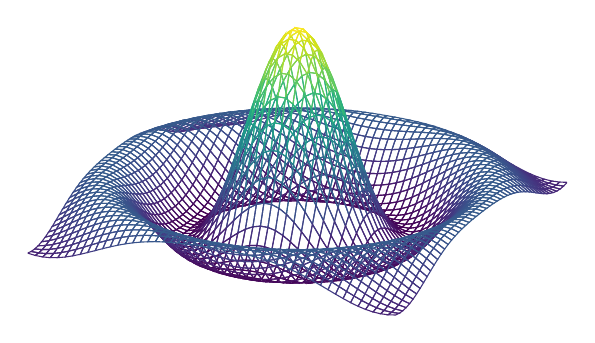
\begin{tikzpicture}
        \begin{axis}[
                hide axis,
                colormap/viridis,
            ]
            \addplot3[
                mesh,
                samples=50,
                domain=-8:8,
            ]
            {sin(deg(sqrt(x^2+y^2)))/sqrt(x^2+y^2)};
            %\addlegendentry{\(\frac{sin(r)}{r}\)}
        \end{axis}
    \end{tikzpicture}
    \caption{Exemple de graphique 3D avec PGF Plots}
\end{figure}

\subsection{Jonction semiconducteur}

Voici un autre exemple d'un diagramme de jonction semi-conducteur.

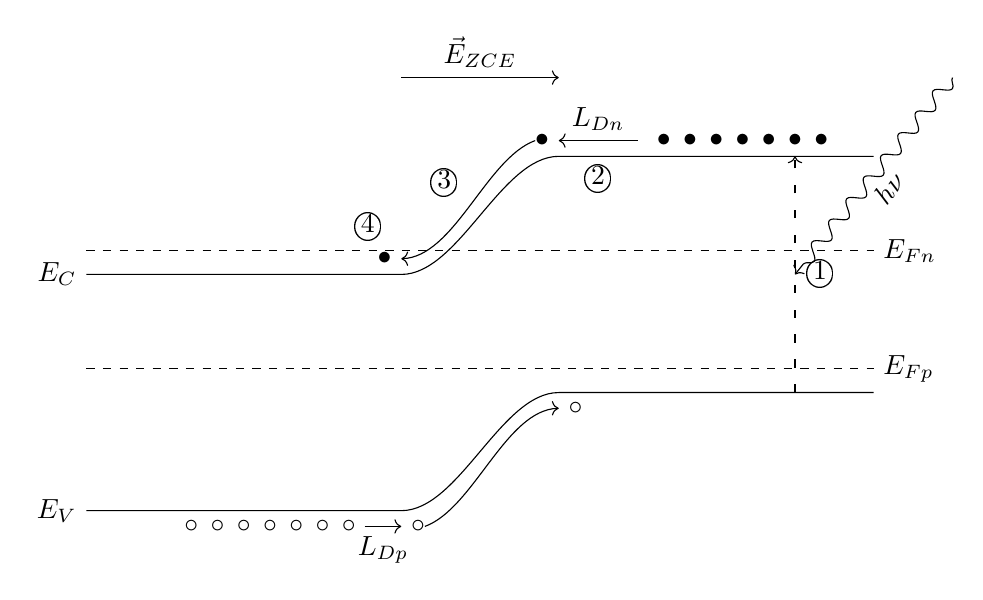
\begin{tikzpicture}
    % variables for pn-junction diagram:
    % all parameters are in tikz scale
    % p-side of the junction is here on the right

    \def\V{1.5}   % junction polarisation (0=flat band)
    \def\EG{3}    % band gap of semiconductor
    \def\EF{1.5}  % vertical Fermi level position
    \def\EFn{3.3} % pseudo fermi level for electrons
    \def\EFp{1.8} % pseudo fermi level for holes
    \def\DZCE{4}  % start position on the left for space charge region (SCR)
    \def\LZCE{2}  % SCR width
    \def\PN{10}   % total lentgh of the junction

    % calculations
    \pgfmathsetmacro\EC{\EG+\V};% conduction band heigth (without polarisation)
    \pgfmathsetmacro\FZCE{\DZCE+\LZCE};% SCR end position

    % valence and conduction band drawing:
    \draw (0,0) node [left]{$E_V$} -- (\DZCE,0)
    to[out=0, in=180, looseness=0.75] (\FZCE,\V) -- (\PN,\V); % EV
    \draw (0,\EG) node [left] {$E_C$} -- (\DZCE,\EG)
    to[out=0, in=180, looseness=0.75] (\FZCE,\EC) -- (\PN,\EC); % EC

    % fermi level drawing (if needed):
    %	\draw [dashed](0,\EF) -- ({\PN-0.5},\EF) node [right]{$E_F$}; % EF

    % quasi fermi levels drawing (if needed) :
    \draw [dashed] (0,\EFn)  -- (\PN,\EFn)
    node [right] {$E_{Fn}$}; % EFn for electron
    \draw [dashed] (0,\EFp)  -- ({\PN},\EFp)
    node [right] {$E_{Fp}$}; % EFp for holes

    % electric field in SCR drawing :
    \draw [->] (\DZCE, {\V+\EG+1}) --
    node [above] {$\vec{E}_{ZCE}$} (\FZCE, {\V+\EG+1}) ; % E vector

    % excess carriers
    \foreach \x in {1,2,...,7}
    \draw ({\FZCE+1+\x/3},{\EC+0.2}) node {$\bullet$}; % p side : electrons
    \foreach \x in {1,2,...,7}
    \draw ({1+\x/3},{-0.2}) node {$\circ$}; % n side : holes

    % photon injection and carrier generation
    % p side : carrier generation:
    \draw [->, loosely dashed] ({\FZCE+3}, \V) --
    node [right] {\textcircled{1}}({\FZCE+3}, \EC);
    % the textcircled{number} option is used in several places
    % to describe the physical mechanisms.
    % It can be safely removed if not needed
    % photon wave injection in the bandgap on p-side :
    \draw [decorate, decoration={snake}, ->] ({\PN+1},{\EC+1}) --
    node [below,sloped]{$h\nu$} ({\FZCE+3}, \EG);

    % excess carriers diffusion, with diffusion length :
    % electrons on p side :
    \draw [->] ({\FZCE+1},{\EC+0.2}) -- node [above] {$L_{Dn}$}
    node [below=6pt] {\textcircled{2}}({\FZCE},{\EC+0.2})
    node [left] {$\bullet$} ;
    \draw [->] ({\FZCE-0.3},{\EC+0.2}) to [out=200, in=0, looseness=0.75]
    node [above left] {\textcircled{3}} ({\DZCE},{\EG+0.2})
    node [left] {$\bullet$} node [above left=3pt] {\textcircled{4}};
    % holes on n side :
    \draw [->] ({1.2+7/3},{-0.2}) -- node [below] {$L_{Dp}$} ({\DZCE},{-0.2})
    node [right]{$\circ$} ;
    \draw [->] ({\DZCE+0.3},-0.2) to [out=20, in=180, looseness=0.75]
    ({\FZCE},{\V-0.2}) node [right]{$\circ$};
\end{tikzpicture}

\subsection{Moteur à combustion}

Voici un exemple d'un modèle d'un papillon des gaz utilisé dans un moteur à combustion interne. Le système mécatronique est modélisé par des sous-systèmes simplifiés permettant une description plus facile. Ce modèle a été utilisé dans le cadre d'un projet étudiant à l'Université technique de Berlin.

\begin{circuitikz}
    %	\draw [help lines] (-1,-2) grid (12,5);

    % electrical equivalent circuit
    \draw (0,3) to[V, v_=$U_R$] (0,0);
    \draw (0,3) to[R, i>^=$I_A$, l=$R_A$] (3,3);
    \draw (3,3) to[L, l=$L_A$] (4,3);

    \draw (4,3) -- (5,3);
    \draw (5,3) to[V, v_=$U_i$] (5,0);
    \draw (0,0) -- (5,0);

    % drive
    \draw[fill=black] (4.85,0.85) rectangle (5.15,2.15);
    \draw[fill=white] (5,1.5) ellipse (.45 and .45);

    % transmission gear one
    \draw[fill=black!50] (6.7,1.49)
    ellipse (.08 and 0.33);
    \draw[fill=black!50, color=black!50] (6.7,1.82)
    rectangle (6.5,1.16);
    \draw[fill=white] (6.5,1.49)
    ellipse (.08 and 0.33);
    \draw (6.5,1.82) -- (6.7,1.82);
    \draw (6.5,1.16) -- (6.7,1.16);

    % shaft drive -> transmission
    \draw[fill=black] (5.45,1.45) rectangle (6.5,1.55);

    % momentum arrow of drive -> transmission
    \draw[line width=0.7pt,<-] (5.8,1) arc (-30:30:1);

    % transmission gear two
    \draw[fill=black!50] (6.7,0.40)
    ellipse (.13 and 0.67);
    \draw[fill=black!50, color=black!50] (6.7,1.07)
    rectangle (6.5,-0.27);
    \draw[fill=white] (6.5,0.40)
    ellipse (.13 and 0.67);
    \draw (6.5,1.07) -- (6.7,1.07);
    \draw (6.5,-0.27) -- (6.7,-0.27);

    % transmission gear three
    \draw[fill=black!50] (6.85,1.14)
    ellipse (.08 and 0.3);
    \draw[fill=black!50, color=black!50] (6.85,1.44)
    rectangle (6.65,0.84);
    \draw[fill=white] (6.65,1.14)
    ellipse (.08 and 0.3);
    \draw (6.65,1.44) -- (6.86,1.44);
    \draw (6.65,0.84) -- (6.86,0.84);

    % transmission shaft from gear two to moment of inertia
    \draw[fill=black] (6.84,0.38) rectangle (7.8,0.48);

    % moment of inertia
    \draw[fill=white] (8.5,0.42)
    ellipse (.15 and 0.4);
    \draw[fill=white, color=white] (7.9, 0.82)
    rectangle (8.49, 0.02);
    \draw (7.8,0.42) ellipse (.15 and 0.4);
    \draw (7.8,0.82) -- (8.5,0.82);
    \draw (7.8,0.02) -- (8.5,0.02);

    % momentum arrow between transmission and moment of inertia
    \draw[line width=0.7pt,<-] (7.2,-0.07) arc (-30:30:1);

    % shaft right from moment of inertia
    \draw[fill=black] (8.65,0.38) rectangle (10.9,0.48);

    % brake shoe
    \draw[fill=black] (9.55,{0.53+0.00})
    -- +(-0.2,0.3) -- +(0.5,0.3) -- +(0.3,0.0);
    \draw[fill=black] (9.55,{0.33-0.00})
    -- +(-0.2,-0.3) -- +(0.5,-0.3) -- +(0.3,0.0);

    % momentum arrow (left hand side of brake shoe)
    \draw[line width=0.7pt,->] (9.05,-0.07) arc (-30:30:1);

    % spring
    \draw [domain=0:{-4.5*pi}, variable=\t, samples=200,
        line width=1pt]
    plot( {10.52+0.4 + 0.15*(\t*0.1)*cos(\t r)},
    {0.40 + 0.15*(\t*0.3)*sin(\t r)});

    % momentum arrow (left hand side of spring)
    \draw[line width=0.7pt,->] (10.4,-0.07) arc (-30:30:1);

    % spring wall mount
    \draw[fill=black]
    (10.9,{1.03-0.2}) rectangle (10.95,{1.03+0.2});
    \foreach \x in {0,...,5}
    \draw[line width=0.8pt]
    ({10.55+0.4},{1.03-0.18+\x*0.07}) -- +(0.1,0.05);

    % descriptions inside graphic
    \draw (5.85,2.2) node {$\omega_A, M_A$};
    \draw (7.29,1.11) node {$\omega_K$};
    \draw (8.25,0.44) node {$J$};
    \draw (9.05,1.15) node {$M_R$};
    \draw (10.4,1.15) node {$M_F$};
    \draw (6.6,-0.5) node {$v$};

    % descriptions of subsystems under graphic
    \draw [decorate,decoration={brace,amplitude=10pt},
        xshift=0pt, yshift=0pt]
    (5.5,-0.75) -- (-0.5,-0.75)
    node[black,midway,yshift=-20pt]
    {Sous-système électromagnétique};
    \draw [decorate,decoration={brace,amplitude=10pt},
        xshift=0pt, yshift=0pt]
    (11.4,-0.75) -- (6,-0.75)
    node[black,midway,yshift=-20pt]
    {Sous-système mécanique};
\end{circuitikz}

\subsection{Schéma électronique}

Vous pouvez également utiliser TikZ pour créer vos propres schémas électriques et électroniques comme l'exemple \ref{circuit}.

\begin{figure}[ht]
    \begin{center}
        \begin{circuitikz}
            \draw
            (0,0) to [short, *-] (6,0)
            to [V, l_=$\mathrm{j}{\omega}_m \underline{\phi}^s_R$] (6,2)
            to [R, l_=$R_R$] (6,4)
            to [short, i_=$\underline{i}^s_R$] (5,4)
            (0,0) to [open, v^>=$\underline{u}^s_s$] (0,4)
            to [short, *- ,i=$\underline{i}^s_s$] (1,4)
            to [R, l=$R_s$] (3,4)
            to [L, l=$L_{\sigma}$] (5,4)
            to [short, i_=$\underline{i}^s_M$] (5,3)
            to [L, l_=$L_M$] (5,0);
        \end{circuitikz}
        \caption{Circuit électrique \label{circuit}}
    \end{center}
\end{figure}

\chapter{Conclusion}
\chapter{Conclusion}

On dénote deux type de conclusion : la conclusion technique et la conclusion personnelle. La conclusion est la deuxième partie qui sera lue par un manager de société après le résumé. Elle doit être concise et claire. Elle doit résumer les résultats obtenus et dresser une conclusion objective du projet. La conclusion technique doit être basée sur les résultats obtenus et doit être en lien avec les objectifs fixés. La conclusion personnelle est une réflexion personnelle sur le projet. Elle peut contenir des éléments qui n'ont pas été abordés dans le rapport, des éléments qui ont été appris durant le projet, des éléments qui ont été appréciés ou non, etc.

Bien entendu vous pouvez également donner un sens plus intime en parlant de votre ressenti, de ce que vous avez appris, de ce que vous avez aimé ou non, etc. C'est une manière de donner une touche personnelle à votre travail.

Il peut être coutume de signer la conclusion encore que votre rapport comporte déjà votre signature numérique. Cela reste un choix personnel.

\vfil
\hspace{8cm}\makeatletter\@author\makeatother\par
\hspace{8cm}\begin{minipage}{5cm}
    % Place pour signature numérique
    \printsignature
\end{minipage}

\clearpage
\printbibliography

\appendix
\appendixpage
\addappheadtotoc



\let\cleardoublepage\clearpage
\backmatter

\label{glossaire}
\printnoidxglossary
\label{index}
\printindex

% Le colophon est le dernier élément d'un document qui contient des notes de l'auteur concernant la mise en page et l'édition du document : il est parfaitement optionnel.
%%if
\clearpage
\Large\textbf{Colophon :}\par\normalsize
\thispagestyle{empty}
La qualité de cet ouvrage repose que le moteur \LaTeX. La mise en page et le format sont inspirés d'ouvrages scientifiques tels que le modèle de thèse de l'EPFL et celui des publications O'Reilly.

Les diagrammes et les illustrations sont édités depuis l'outil en ligne draw.io. Certaines illustrations ont été reprises dans Adobe Illustrator. Les représentations 3D sont exportées de SolidWorks et certains graphiques sont générés à la volée depuis un code source Python.

L'auteur fictive de ce document \emph{Maria Bernasconi} est un nom emprunté, par amusement, aux spécimens publiés par Postfinance.

Ce document a été compilé avec XeLaTeX.

La famille de police de caractères utilisée est \emph{Computed Modern} créée par Donald Knuth avec son logiciel METAFONT.
\vfil
Le Colophon est le dernier élément d'un document qui contient des notes de l'auteur concernant la mise en page et l'édition du document : il est parfaitement optionnel.
%%fi

\end{document}
